\documentclass{article}
\usepackage[utf8]{inputenc}
\usepackage{graphicx}
\usepackage{amsmath, amssymb}
\title{Simulation - chapter 5, even exercises}
\author{Pinak Mandal}
\date{}

\begin{document}

\subsection*{Problem 2}
The distribution function is given by
\begin{align*}
  F(x) = \begin{cases}
            \frac{(x-2)^2}{4}, & 2\le x\le 3 \\
            -\frac{x^2}{12} + x - 2, & 3\le x\le 6
        \end{cases}
\end{align*}
The inverse to which is given by
\begin{align*}
  F^{-1}(y) = \begin{cases}
                2(\sqrt{y}+1), & 0\le y\le \frac{1}{4}\\
                6-2\sqrt{3(1-y)}, & \frac{1}{4}\le y\le 1
              \end{cases}
\end{align*}
$1000$ samples generated with inverse transform algorithm yield the following result.
\begin{figure}[h!]
    \centering
    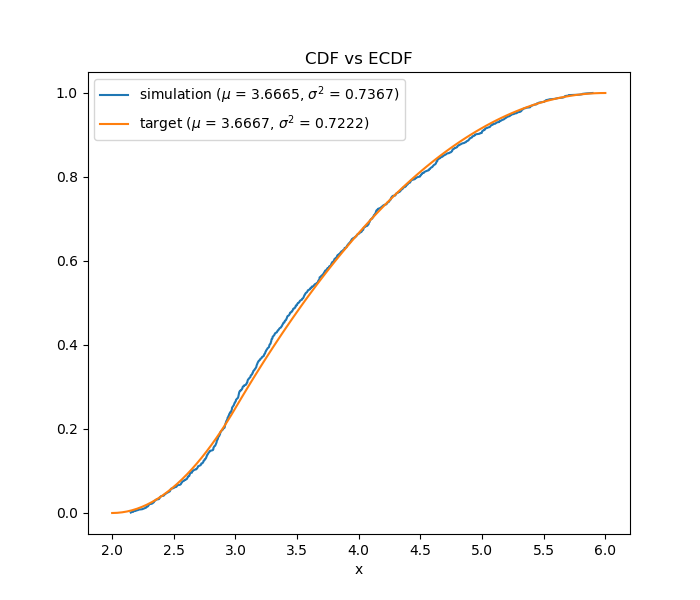
\includegraphics[width=\linewidth]{../images/p2_1000.png}
    \caption{distribution comparison}
\end{figure}
\newpage

\subsection*{Problem 4}
\begin{align*}
  F^{-1}(y) = \left[-\frac{\log(1-y)}{\alpha}\right]^{\frac{1}{\beta}}
\end{align*}
The pdf is given by
\begin{align*}
  f(x) = \alpha\beta\,x^{\beta-1}\exp(-\alpha x^{\beta})
\end{align*}
The mean is $\frac{1}{\sqrt[\beta]{\alpha}}\Gamma\left(1+\frac{1}{\beta}\right)$ and the variance is $\frac{1}{\sqrt[\beta]{\alpha^2}}\left[\Gamma\left(2+\frac{1}{\beta}\right)-\Gamma\left(1+\frac{1}{\beta}\right)^2\right]$.
$1000$ samples generated with inverse transform algorithm yield the following result.
\begin{figure}[h!]
    \centering
    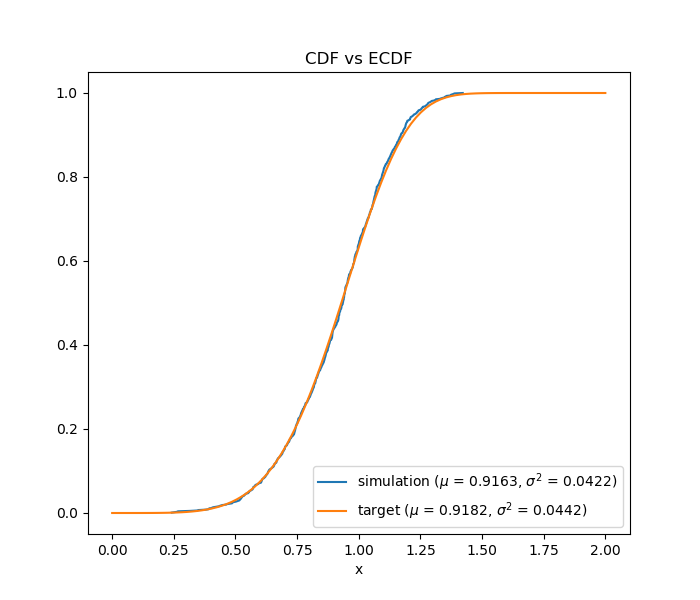
\includegraphics[width=\linewidth]{../images/p4_1_5_1000.png}
    \caption{distribution comparison for $\alpha = 1,\,\beta = 5$}
\end{figure}
\newpage

\subsection*{Problem 6}
The inverse of the cdf is given by
\begin{align*}
  F^{-1}(y) = -\log(1-cy), \;\; c = 1 - e^{-0.05}
\end{align*}
Mean of the target distribution is given by,
\begin{align*}
  \frac{1-1.05e^{-0.05}}{1-e^{-0.05}}
\end{align*}
$1000$ samples generated with inverse transform algorithm yield the following result.
\begin{figure}[h!]
    \centering
    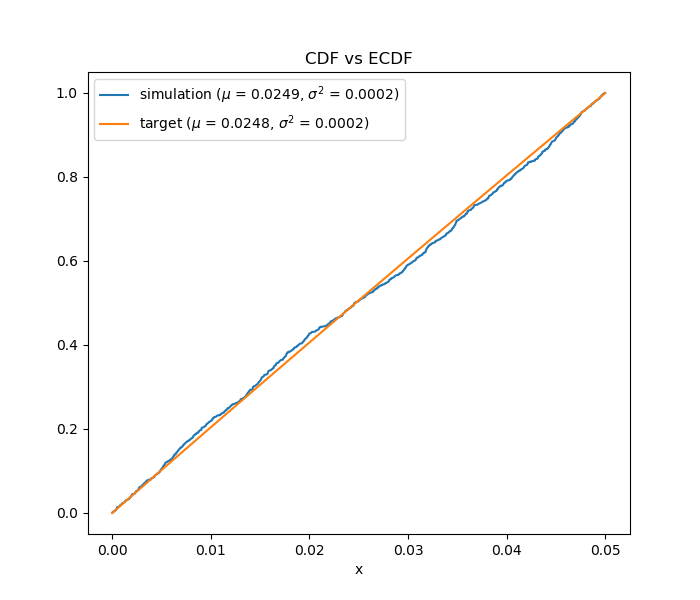
\includegraphics[width=\linewidth]{../images/p6.png}
    \caption{distribution comparison}
\end{figure}
\newpage

\subsection*{Problem 8(a)}
The inverse of $F_{i}(x)$ is given by
\begin{align*}
  F_{i}^{-1}(y)=y^{\frac{1}{2i-1}}, \;\; i=1,2,3
\end{align*}
$1000$ samples generated with composition method yield the following result.
\begin{figure}[h!]
    \centering
    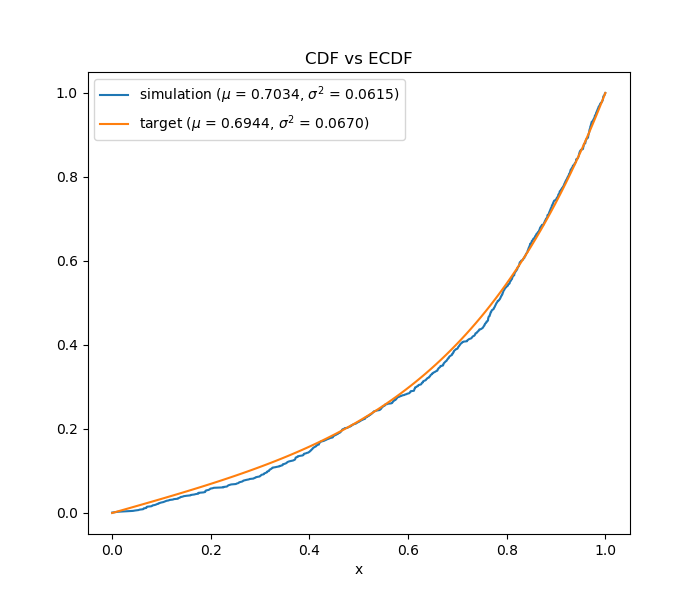
\includegraphics[width=\linewidth]{../images/p8a_1000.png}
    \caption{distribution comparison}
\end{figure}
\newpage

\subsection*{Problem 8(b)}
Our setup is as follows.
\begin{align*}
  F_1(x) &= 1-e^{-2x},\;\; 0< x< \infty\\
  F_2(x) &= \begin{cases}
              x, & 0< x< 1\\
              1, & 1\le x<\infty
            \end{cases}\\
  F(x) &= \frac{1}{3}F_{1}(x) + \frac{2}{3}F_{2}(x)\\
\end{align*}
$1000$ samples generated with composition method yield the following result.
\begin{figure}[h!]
    \centering
    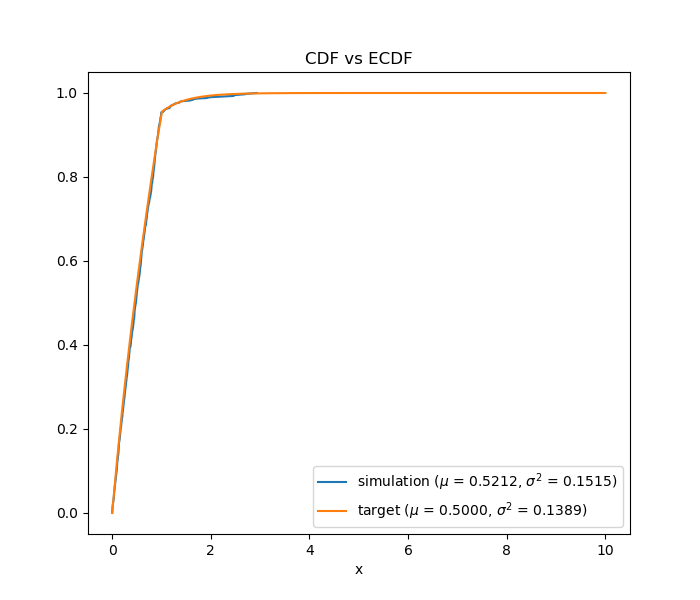
\includegraphics[width=\linewidth]{../images/p8b_1000.png}
    \caption{distribution comparison}
\end{figure}
\newpage

\subsection*{Problem 8(c)}
Our setup is as follows. The probability weights have been generated randomly.
\begin{align*}
  \bar\alpha = ( & 0.17681302, 0.08941652, 0.13690479, 0.14830053, 0.15965611, \\
                 & 0.17054088, 0.03269305, 0.00496038, 0.0506282,  0.03008653)
\end{align*}
$1500$ samples generated with composition method yield the following result.
\begin{figure}[h!]
    \centering
    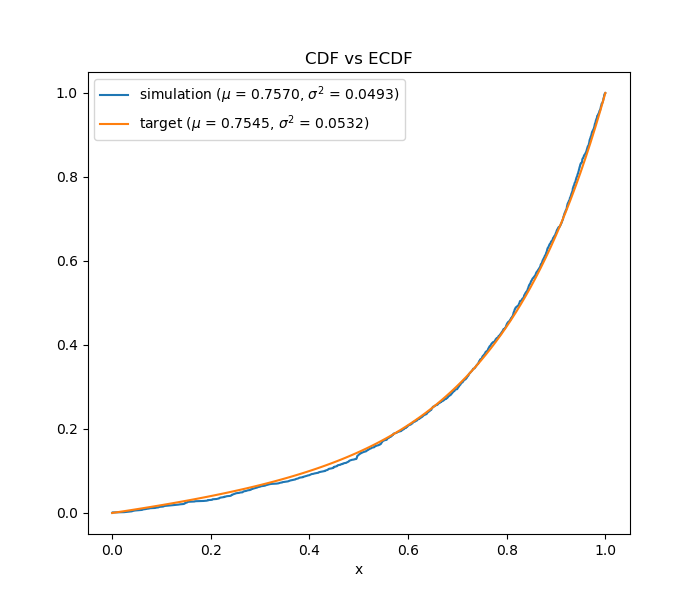
\includegraphics[width=\linewidth]{../images/p8c_10_1500.png}
    \caption{distribution comparison}
\end{figure}
\newpage

\subsection*{Problem 10}
Our notation is as follows.
\newline
$n = 1000 = $ number of policyholders
\newline
$s_i = $ indicator variable for $i$-th policyholder presenting a claim
\newline
$p = E[s_i] = 0.05\;\forall i$
\newline
$X_i = $ amount of claim presented by $i$-th policyholder
\newline
$\mu = E[X_i] = \$\, 800\;\forall i$
\newline
$Y = \sum_{i=1}^n s_i X_i$ = amount of total claim presented by all policyholders
\newline
$F(x) = $ cdf of $Y$
\newline
$A = \$\,50,000$
\newline
$M$ = set of all binary $n$-tuples
\newline
$M_k = $  set of binary $n$-tuple with exactly $k$-entries being $1$
\newline
$P(Y > A|m) = $ probability conditioned on $s_i=m_i\;\forall i$ where $m\in M$.
\newline
$P(m) = $ probability that $s_i = m_i\;\forall i$ where $m\in M$.
\newline
$\Gamma(x, k, \mu) = $ cdf of gamma random variable that is the sum of $k$ identical exponential random variables with mean $\mu$
\newline
With our notations we need to compute the following.
\begin{align*}
F(A) =& \,P(Y \le A) = \sum_{m\in M}P(Y \le A| m)P(m) \\
=& \sum_{k=1}^n\sum_{m\in M_k}P(Y \le A| m)P(m) \\
=& \sum_{k=1}^n\sum_{m\in M_k}P(Y \le A| m)p^k(1-p)^{n-k} \\
=& \sum_{k=1}^n |M_k|p^k(1-p)^{n-k} P(Y \le A| m_k) ,\qquad m_k\in M_k \\
=& \sum_{k=1}^n \binom{n}{k}p^k(1-p)^{n-k}P(Y \le A| m_k) \\
=& \sum_{k=1}^n \binom{n}{k}p^k(1-p)^{n-k}\Gamma(A, k, \mu) \\
=:& \sum_{k=1}^n p_{n,k}\Gamma(A, k, \mu)
\end{align*}
$\sum_{k=1}^n p_{n,k} = 1$ and $p_{n,k} > 0$ which implies we can sample $Y$ using composition technique because we can already sample gamma distributions. $1000$ samples generated using composition technique sets the required probability at $12\% - 13\%$. We can also sample $Y$ by simulating $n$ Bernoulli trials and then simulating $s$ exponential random variables where $s = $ the number of successes in the Bernoulli trials. This straight-forward method sets the required probability at $10\%-12\%$. The actual value of the required probability $\approx 10.7\%$.
\end{document}
